\documentclass[conference]{IEEEtran}
\IEEEoverridecommandlockouts

\usepackage[utf8]{inputenc}
\usepackage[T5]{fontenc}
\usepackage[vietnamese]{babel}
\usepackage{cite}
\usepackage{amsmath,amssymb,amsfonts}
\usepackage{algorithmic}
\usepackage{graphicx}
\usepackage{textcomp}
\usepackage{xcolor}
\usepackage{booktabs}
\usepackage{array}
\usepackage{multirow}
\usepackage{url}

\def\BibTeX{{\rm B\kern-.05em{\sc i\kern-.025em b}\kern-.08em
    T\kern-.1667em\lower.7ex\hbox{E}\kern-.125emX}}

\begin{document}

\title{Phân tích so sánh Minimax cắt tỉa Alpha-Beta và MCTS-UCT cho trò chơi Tic-Tac-Toe}

\author{
\IEEEauthorblockN{Phạm Thiên Minh}
\IEEEauthorblockA{\textit{Trường Đại học Công nghệ} \\
\textit{Đại học Quốc gia Hà Nội (UET-VNU)}\\
Hà Nội, Việt Nam}
\and
\IEEEauthorblockN{Lục Gia Bảo}
\IEEEauthorblockA{\textit{Trường Đại học Công nghệ} \\
\textit{Đại học Quốc gia Hà Nội (UET-VNU)}\\
Hà Nội, Việt Nam}
}

\IEEEaftertitletext{\vspace{-1.2\baselineskip}\begin{center}\textit{Ghi chú: Thành viên Nguyễn Khắc Trọng hiện đang nghỉ học tạm thời nên không tham gia thực hiện bài tập lớn này.}\end{center}\vspace{0.6\baselineskip}}

\maketitle

\begin{abstract}
Báo cáo trình bày việc cài đặt và so sánh thực nghiệm hai thuật toán tìm kiếm cây trò chơi kinh điển---Minimax với cắt tỉa Alpha-Beta và Tìm kiếm cây Monte Carlo kết hợp UCT (MCTS-UCT)---trên cả bàn cờ Tic-Tac-Toe $3\times 3$ cổ điển và bàn cờ $15\times 15$ năm quân thẳng hàng (Gomoku / Cờ caro). Cắt tỉa Alpha-Beta giúp giảm $71{,}8\%$ số nút duyệt của Minimax ở độ sâu $4$ trên bàn $3\times 3$ và giảm $88{,}0\%$ ở độ sâu $3$ trên bàn $15\times 15$ mà không làm thay đổi nước đi được chọn. Trên bàn $3\times 3$, MCTS-UCT với $\ge 1000$ vòng lặp đạt $0$ ván thua qua $50$ ván đổi lượt đi trước khi đấu với cả tác tử ngẫu nhiên lẫn đối thủ Alpha-Beta tối ưu ở độ sâu $9$. Khi khảo sát hằng số khám phá $c \in \{0{,}5;\ 1{,}0;\ 1{,}4;\ 2{,}0\}$, giá trị $c = 0{,}5$ hội tụ nhanh nhất khi ngân sách vòng lặp thấp trên bàn $15\times 15$ (tỷ lệ thắng $100\%$ ở $200$ vòng lặp), trong khi $c \in \{1{,}0;\ 1{,}4\}$ đạt $100\%$ ($50/50$) ở $500$ vòng lặp. Thay thế mô phỏng ngẫu nhiên bằng mô phỏng heuristic chiến thuật một bước giúp tăng tỷ lệ thắng thêm $+6{,}0\%$ trên bàn $3\times 3$ ($84{,}0\% \rightarrow 90{,}0\%$) và $+16{,}0\%$ trên bàn $15\times 15$ ($76{,}0\% \rightarrow 92{,}0\%$), minh họa nguyên lý nền tảng của mạng giá trị (value network) và mạng chính sách (policy network) trong các hệ thống hiện đại như AlphaGo. Báo cáo cũng trình bày cơ sở toán học của UCT từ bài toán Multi-Armed Bandit và giải thích lý do chọn nước đi cuối cùng theo số lần thăm $N$ thay vì tỷ lệ thắng $W/N$.
\end{abstract}

\begin{IEEEkeywords}
Minimax, Cắt tỉa Alpha-Beta, MCTS, UCT, Multi-Armed Bandit, Tic-Tac-Toe, Gomoku
\end{IEEEkeywords}

\section{Giới thiệu}
Tìm kiếm trên cây trò chơi là một nền tảng quan trọng của trí tuệ nhân tạo, với nhiều ứng dụng từ trò chơi đối kháng đến lập kế hoạch và điều độ tự động~\cite{russell2020}. Dù có luật chơi đơn giản, Tic-Tac-Toe là bài toán chuẩn lý tưởng để so sánh giữa tìm kiếm tất định chính xác (Minimax kết hợp cắt tỉa Alpha-Beta) và tìm kiếm ngẫu nhiên theo thời gian thực (MCTS-UCT), đặc biệt khi mở rộng từ bàn $3\times 3$ (3 quân thẳng hàng) lên bàn $15\times 15$ (5 quân thẳng hàng / Gomoku), nơi việc duyệt vét cạn trở nên bất khả thi về mặt tính toán.

Nghiên cứu này tập trung trả lời năm câu hỏi nghiên cứu (RQ):
\begin{itemize}
    \item \textbf{RQ1:} Cắt tỉa Alpha-Beta giảm được bao nhiêu phần trăm số nút duyệt so với Minimax thuần trên bàn $3\times 3$ và $15\times 15$?
    \item \textbf{RQ2:} Hằng số khám phá $c \in \{0{,}5;\ 1{,}0;\ 1{,}4;\ 2{,}0\}$ trong UCT ảnh hưởng thế nào đến tỷ lệ thắng theo số vòng lặp?
    \item \textbf{RQ3:} MCTS-UCT có thực sự không bao giờ thua trên bàn $3\times 3$ hay không, và điều này đạt được từ ngưỡng vòng lặp nào?
    \item \textbf{RQ4:} Mô phỏng heuristic cải thiện MCTS bao nhiêu so với mô phỏng ngẫu nhiên, và đánh đổi về thời gian chạy ra sao?
    \item \textbf{RQ5:} Vì sao nước đi cuối cùng nên được chọn theo số lần thăm $N$ lớn nhất thay vì tỷ lệ thắng thực nghiệm $W/N$?
    \item \textbf{RQ6 (Mở rộng):} Các biến thể công thức UCT (bỏ $\sqrt{\cdot}$, bỏ $\ln$, hoặc bỏ cả hai) và cải tiến Progressive Bias ảnh hưởng thế nào đến hiệu năng tìm kiếm?
\end{itemize}

\section{Phát biểu bài toán}
Trò chơi được mô hình hóa như một trò chơi hai người, tổng bằng không, tất định và thông tin đầy đủ:
\begin{itemize}
    \item \textbf{Trạng thái $s$:} Lưới $n \times n$ với mỗi ô nhận giá trị trong $\{X (+1), O (-1), \emptyset (0)\}$, trong đó $X$ đi trước.
    \item \textbf{Hành động $a$:} Đặt quân của người chơi hiện tại vào một ô trống. Để giữ không gian tìm kiếm khả thi trên bàn $15\times 15$, hàm \texttt{get\_legal\_moves()} giới hạn các nước ứng viên trong vùng lân cận khoảng cách Chebyshev $\text{radius} = 2$ quanh các quân đã đặt (và bắt buộc đánh ô trung tâm $(\lfloor n/2 \rfloor, \lfloor n/2 \rfloor)$ khi bàn trống). Bán kính $2$ giúp giữ lại các nước đe dọa cách một ô như \texttt{\_ O \_ O \_}.
    \item \textbf{Điều kiện dừng:} Có $\text{win\_len}$ quân liên tiếp theo hàng ngang, cột dọc hoặc đường chéo ($3$ trên bàn $3\times 3$; $5$ trên bàn $15\times 15$), hoặc bàn cờ đầy (hòa).
    \item \textbf{Hàm lợi ích:} Với Minimax/Alpha-Beta là $+1{,}000{,}000$ (thắng), $-1{,}000{,}000$ (thua), $0$ (hòa), hoặc điểm lượng giá $\text{eval}(s, p)$ khi chạm giới hạn độ sâu. Với MCTS-UCT là $1{,}0$ (thắng), $0{,}5$ (hòa hoặc mô phỏng bị cắt), và $0{,}0$ (thua), nằm trong đoạn $[0, 1]$ theo yêu cầu của UCB1.
\end{itemize}

\section{Phương pháp}

\subsection{Minimax cắt tỉa Alpha-Beta và Hàm lượng giá}
Minimax thực hiện tìm kiếm theo chiều sâu (DFS) đến giới hạn $\text{max\_depth}$, giả định cả hai bên đều chơi tối ưu:
\begin{equation}
V(s, d) =
\begin{cases}
\text{eval}(s, \text{me}), & \text{terminal}(s) \text{ hoặc } d = 0 \\
\max_{a \in A(s)} V(s', d - 1), & \text{lượt MAX} \\
\min_{a \in A(s)} V(s', d - 1), & \text{lượt MIN}
\end{cases}
\end{equation}
trong đó $s' = T(s, a)$ là trạng thái sau khi thực hiện nước đi $a$. Alpha-Beta duy trì hai cận---$\alpha$ (điểm tốt nhất đảm bảo cho MAX) và $\beta$ (điểm tốt nhất đảm bảo cho MIN)---và cắt bỏ nhánh con ngay khi $\alpha \ge \beta$. Với thứ tự duyệt nước tối ưu, độ phức tạp thời gian giảm từ $\mathcal{O}(b^d)$ xuống $\mathcal{O}(b^{d/2})$, tương đương tăng gấp đôi độ sâu tìm kiếm hiệu dụng.

\textbf{Hàm lượng giá heuristic (\texttt{evaluate}):} Tại các nút lá chưa kết thúc khi hết độ sâu, bàn cờ được quét theo cả bốn hướng (ngang, dọc, chéo chính, chéo phụ). Với mỗi chuỗi quân liên tiếp độ dài $L$ của người chơi $p$, thuật toán đếm số ô trống ở hai phía ($\text{space\_left}$, $\text{space\_right}$). Nếu $L + \text{space\_left} + \text{space\_right} < \text{win\_len}$, chuỗi bị chặn hoàn toàn và nhận $0$ điểm. Ngược lại, $\text{open\_ends} \in \{1, 2\}$ đếm số đầu kề ô trống (giới hạn tối đa $1$ nếu tổng chỗ trống vừa đúng bằng $\text{win\_len}$), và mẫu quân được chấm điểm phi tuyến theo Bảng~\ref{tab:eval_weights}. Giá trị lượng giá cuối cùng là $\text{total\_score}(\text{me}) - \text{total\_score}(\text{opponent})$. Thang điểm tăng theo cấp số nhân ép Minimax ưu tiên tạo hoặc chặn chuỗi $4$ mở thay vì tích lũy các chuỗi $2$ nhỏ lẻ, còn hệ số $10\times$ cho chuỗi mở $2$ đầu phản ánh việc đối thủ chỉ có thể chặn một đầu trong một lượt.

\begin{table}[t]
\centering
\caption{Bảng trọng số mẫu quân trong hàm lượng giá}
\label{tab:eval_weights}
\begin{tabular}{@{}ccrl@{}}
\toprule
Độ dài & Số đầu mở & Điểm & Ý nghĩa chiến thuật \\
\midrule
5 & 1 hoặc 2 & 100.000 & Chuỗi thắng \\
4 & 2 & 50.000 & Nước đôi gần như thắng chắc \\
4 & 1 & 5.000 & Đe dọa trực tiếp (chặn được) \\
3 & 2 & 2.000 & Chuỗi 3 mở mạnh ($10\times$ mở 1 đầu) \\
3 & 1 & 200 & Chuỗi 3 mở 1 đầu \\
2 & 2 & 100 & Chuỗi 2 mở 2 đầu \\
2 & 1 & 10 & Chuỗi 2 mở 1 đầu \\
1 & 2 / 1 & 5 / 1 & Ưu tiên vị trí nhỏ \\
\bottomrule
\end{tabular}
\end{table}

\subsection{MCTS + UCT và Cơ sở toán học}
MCTS xây dựng cây tìm kiếm bất đối xứng qua $K$ vòng lặp gồm bốn bước~\cite{coulom2006,kocsis2006}:
\begin{enumerate}
    \item \textbf{Selection (Lựa chọn):} Bắt đầu từ gốc, đi xuống theo \texttt{best\_child(c)} cực đại hóa UCT cho đến khi gặp nút kết thúc hoặc nút chưa mở rộng hết.
    \item \textbf{Expansion (Mở rộng):} Lấy một nước hợp lệ chưa thử và tạo thêm một nút con mới.
    \item \textbf{Simulation (Mô phỏng / Rollout):} Chơi thử từ nút mới bằng \texttt{rollout\_fn} để thu kết quả $r \in \{0{,}0;\ 0{,}5;\ 1{,}0\}$ theo góc nhìn của \texttt{node.player} (người vừa đánh nước dẫn đến \texttt{node}).
    \item \textbf{Backpropagation (Cập nhật ngược):} Đi ngược lên gốc, tăng $N \leftarrow N + 1$, cộng $W \leftarrow W + r$ (trừ nút gốc vì không có nước đi dẫn vào), và đảo góc nhìn $r \leftarrow 1{,}0 - r$ ở mỗi bước lên cha do cha và con là hai đối thủ của nhau.
\end{enumerate}

Công thức chọn nút con $i$ theo UCT là:
\begin{equation}
\text{UCT}_i = \underbrace{\frac{W_i}{N_i}}_{\text{Khai thác}} + c\,\underbrace{\sqrt{\frac{\ln N_{\mathrm{parent}}}{N_i}}}_{\text{Khám phá}}
\label{eq:uct}
\end{equation}
Các nút con chưa từng được thăm ($N_i = 0$) được gán giá trị $+\infty$ để mọi nước hợp lệ đều được thử ít nhất một lần trước khi so sánh UCT.

\textbf{Cơ sở toán học (Multi-Armed Bandit \& UCB1):} Tại mỗi nút trong cây, việc chọn giữa $K$ nước đi hợp lệ là một bài toán Multi-Armed Bandit (MAB) ngẫu nhiên: mỗi nút con $i$ tương ứng với một tay kéo có phần thưởng kỳ vọng thực chưa biết $\mu_i \in [0, 1]$. Auer và cộng sự~\cite{auer2002} đề xuất chính sách UCB1 chọn tay kéo có cận trên tin cậy (upper confidence bound) của $\mu_i$ lớn nhất.

Căn bậc hai và hàm $\ln$ xuất phát trực tiếp từ bất đẳng thức Hoeffding. Với $N_i$ mẫu độc lập cùng phân phối $X_1, \dots, X_{N_i} \in [0, 1]$ có trung bình mẫu $\bar{X}_i = W_i / N_i$ và kỳ vọng thực $\mu_i$:
\begin{equation}
P(\bar{X}_i - \mu_i \ge \epsilon) \le e^{-2 N_i \epsilon^2}, \qquad
P(\mu_i - \bar{X}_i \ge \epsilon) \le e^{-2 N_i \epsilon^2}.
\end{equation}
Đặt xác suất đuôi bằng $N_{\mathrm{parent}}^{-4}$---số mũ nguyên nhỏ nhất bảo đảm khi cộng qua mọi cặp số lần thử $(s, s_i)$ (tối đa $t^2$ cặp) ở bước $t$, chuỗi $\sum_{t=1}^{\infty} t^2 \cdot t^{-4} = \sum_{t=1}^{\infty} t^{-2} = \pi^2/6 < \infty$ hội tụ và giữ phần dư ở mức $\mathcal{O}(1)$---ta thu được:
\begin{equation}
e^{-2 N_i \epsilon^2} = N_{\mathrm{parent}}^{-4} \implies \epsilon = \sqrt{\frac{2 \ln N_{\mathrm{parent}}}{N_i}}.
\end{equation}
Do đó, với xác suất cao, $\mu_i \le W_i/N_i + \sqrt{2 \ln N_{\mathrm{parent}} / N_i}$. Việc chọn tay kéo có cận trên cao nhất thể hiện nguyên lý \emph{lạc quan trước sự bất định}: tử số $\ln N_{\mathrm{parent}}$ tăng chậm hơn tuyến tính giúp các nhánh bị bỏ quên vẫn được quay lại thăm vô hạn lần nhưng với tần suất giảm dần, trong khi $1/\sqrt{N_i}$ thu hẹp khoảng tin cậy khi số mẫu tăng. Auer và cộng sự~\cite{auer2002} chứng minh UCB1 đạt hối tiếc tích lũy (cumulative regret) bậc logarit:
\begin{equation}
R(N) \le \sum_{i:\,\Delta_i > 0} \frac{8 \ln N}{\Delta_i} + \mathcal{O}(1), \qquad \Delta_i = \mu^* - \mu_i,
\end{equation}
khớp với cận dưới tiệm cận Lai--Robbins $\Omega(\ln N)$ sai khác một hằng số. Kocsis và Szepesvári~\cite{kocsis2006} mở rộng đệ quy UCB1 lên cây trò chơi (UCT) và chứng minh thuật toán hội tụ về nước đi tối ưu minimax khi $N \to \infty$. Trong thực tế, hằng số lý thuyết $\sqrt{2} \approx 1{,}414$ giả định phần thưởng dừng và độc lập trong $[0, 1]$; trên cây trò chơi, phân phối phần thưởng rollout thay đổi khi cây mở rộng sâu hơn, nên cần tinh chỉnh $c$ bằng thực nghiệm.

\subsection{Chiến lược mô phỏng (Rollout)}
\begin{itemize}
    \item \textbf{Rollout ngẫu nhiên (\texttt{random\_rollout}):} Chọn ngẫu nhiên đều một nước hợp lệ ở mỗi bước, tối đa $\text{MAX\_ROLLOUT\_STEPS} = 30$ bước. Trên bàn $3\times 3$, ván đấu kết thúc trong $\le 9$ nước nên không bao giờ bị cắt. Trên bàn $15\times 15$, đánh ngẫu nhiên hiếm khi tạo được $5$ quân thẳng hàng trong $30$ nước; các mô phỏng bị cắt trả về $0{,}5$ (chưa phân thắng bại) để giữ thời gian chạy hợp lý và tránh thiên lệch theo tính chẵn lẻ độ sâu.
    \item \textbf{Rollout heuristic (\texttt{heuristic\_rollout}):} Ở mỗi bước mô phỏng (cũng giới hạn $30$ bước), kiểm tra các nước hợp lệ theo thứ tự: (1) đánh ngay nước thắng nếu có; (2) nếu không, chặn nước thắng ngay của đối thủ; (3) nếu không, chọn ngẫu nhiên đều. Bộ lọc chiến thuật một bước này đóng vai trò như một hàm ước lượng chính sách/giá trị nhẹ và là tiền thân khái niệm của mạng chính sách và mạng giá trị trong AlphaGo~\cite{silver2016}.
\end{itemize}

\subsection{Các biến thể UCT và Cải tiến Progressive Bias}
Để kiểm chứng thực nghiệm vai trò của cả $\sqrt{\cdot}$ và $\ln$ trong công thức~\eqref{eq:uct} đồng thời cải thiện hiệu năng ở ngân sách thấp trên bàn $15\times 15$, chúng tôi đánh giá bốn biến thể rút gọn cùng công thức cải tiến Progressive Bias~\cite{chaslot2008}:
\begin{itemize}
    \item \textbf{UCT chuẩn:} $W_i/N_i + c\sqrt{\ln N_{\mathrm{parent}} / N_i}$.
    \item \textbf{Bỏ căn (No-sqrt):} $W_i/N_i + c\,(\ln N_{\mathrm{parent}} / N_i)$.
    \item \textbf{Bỏ $\ln$ (No-ln):} $W_i/N_i + c\sqrt{N_{\mathrm{parent}} / N_i}$.
    \item \textbf{Tuyến tính (Linear):} $W_i/N_i + c\,(N_{\mathrm{parent}} / N_i)$.
    \item \textbf{Progressive Bias (UCT cải tiến):}
    \begin{equation}
    \text{UCT}_{\mathrm{PB}}(i) = \frac{W_i}{N_i} + c\sqrt{\frac{\ln N_{\mathrm{parent}}}{N_i}} + \frac{H_i}{N_i + 1},
    \end{equation}
    trong đó $H_i = \frac{1}{2}\bigl(1 + \tanh(\text{eval}(s_i, p_i)/5000)\bigr) \in (0, 1)$ được tính một lần và lưu cache trên nút. Khi $N_i \to \infty$, $H_i/(N_i+1) \to 0$, giữ nguyên tính tối ưu tiệm cận của UCT nhưng định hướng tốt hơn ở giai đoạn đầu trên bàn lớn.
\end{itemize}

\section{Thiết lập thực nghiệm}
Toàn bộ thực nghiệm được chạy trên Python 3.14 (NumPy, Matplotlib) với CPU 12 nhân, sử dụng các tiến trình song song (\texttt{ProcessPoolExecutor}), seed cố định theo từng ván và đổi lượt đi trước luân phiên ($X$ ở ván chẵn, $O$ ở ván lẻ) để loại bỏ lợi thế đi trước. Bảng~\ref{tab:setup} tóm tắt các cấu hình thực nghiệm.

\begin{table}[t]
\centering
\caption{Tóm tắt các cấu hình thực nghiệm}
\label{tab:setup}
\setlength{\tabcolsep}{3.5pt}
\begin{tabular}{@{}llll@{}}
\toprule
Thí nghiệm & Bàn cờ & Đối thủ & Số ván \\
\midrule
Minimax vs AB & $3\times 3$, $15\times 15$ & Thế cờ cố định & 1 thế cờ \\
MCTS $c \times$ iters & $3\times 3$ & Random & 100 \\
MCTS $c \times$ iters & $15\times 15$ & Random & 50 \\
Kiểm chứng không thua & $3\times 3$ & AB (d=9), Rand & 50 \\
So sánh Rollout & $3\times 3$ / $15\times 15$ & Random & 100 / 50 \\
Biến thể UCT & $3\times 3$ / $15\times 15$ & AB (d=9), Rand & 100 / 50 \\
\bottomrule
\end{tabular}
\end{table}

\section{Kết quả}

\subsection{Minimax vs Alpha-Beta: Số nút duyệt}
Bảng~\ref{tab:minimax_ab} và Hình~\ref{fig:nodes_3x3}--\ref{fig:nodes_15x15} so sánh số nút duyệt giữa Minimax thuần và cắt tỉa Alpha-Beta. Trên bàn $3\times 3$, Alpha-Beta giảm $71{,}8\%$ số nút ở độ sâu $4$; trên bàn $15\times 15$, mức giảm đạt $88{,}0\%$ ở độ sâu $3$ ($85.290 \rightarrow 10.257$ nút).

\begin{table}[t]
\centering
\caption{Số nút duyệt: Minimax thuần vs Cắt tỉa Alpha-Beta}
\label{tab:minimax_ab}
\begin{tabular}{@{}ccrrr@{}}
\toprule
Bàn cờ & Độ sâu & Minimax & Alpha-Beta & Mức giảm \\
\midrule
$3\times 3$ & 1 & 7 & 7 & 0,0\% \\
$3\times 3$ & 2 & 49 & 32 & 34,7\% \\
$3\times 3$ & 3 & 259 & 132 & 49,0\% \\
$3\times 3$ & 4 & 979 & 276 & \textbf{71,8\%} \\
\midrule
$15\times 15$ & 1 & 36 & 36 & 0,0\% \\
$15\times 15$ & 2 & 1.634 & 410 & 74,9\% \\
$15\times 15$ & 3 & 85.290 & 10.257 & \textbf{88,0\%} \\
\bottomrule
\end{tabular}
\end{table}

\begin{figure}[t]
\centering
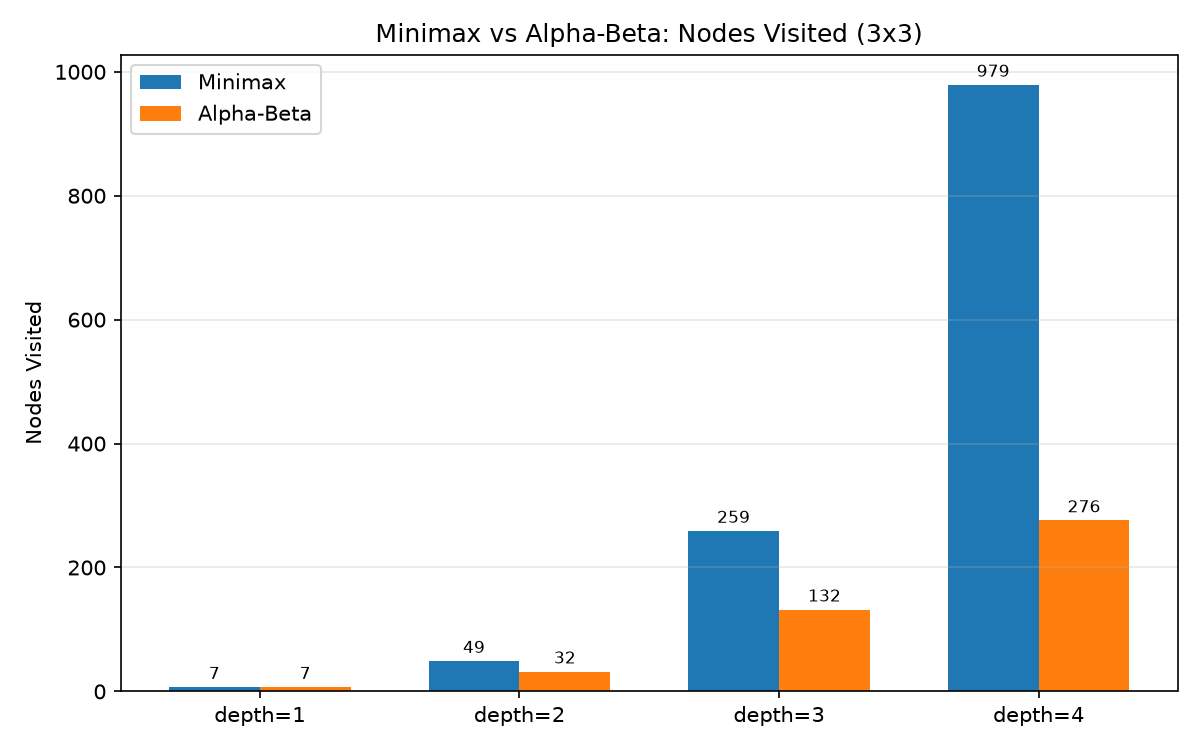
\includegraphics[width=0.95\linewidth]{../assets/figures/nodes_minimax_vs_ab_3x3.png}
\caption{So sánh số nút duyệt trên thế cờ thử nghiệm $3\times 3$.}
\label{fig:nodes_3x3}
\end{figure}

\begin{figure}[t]
\centering
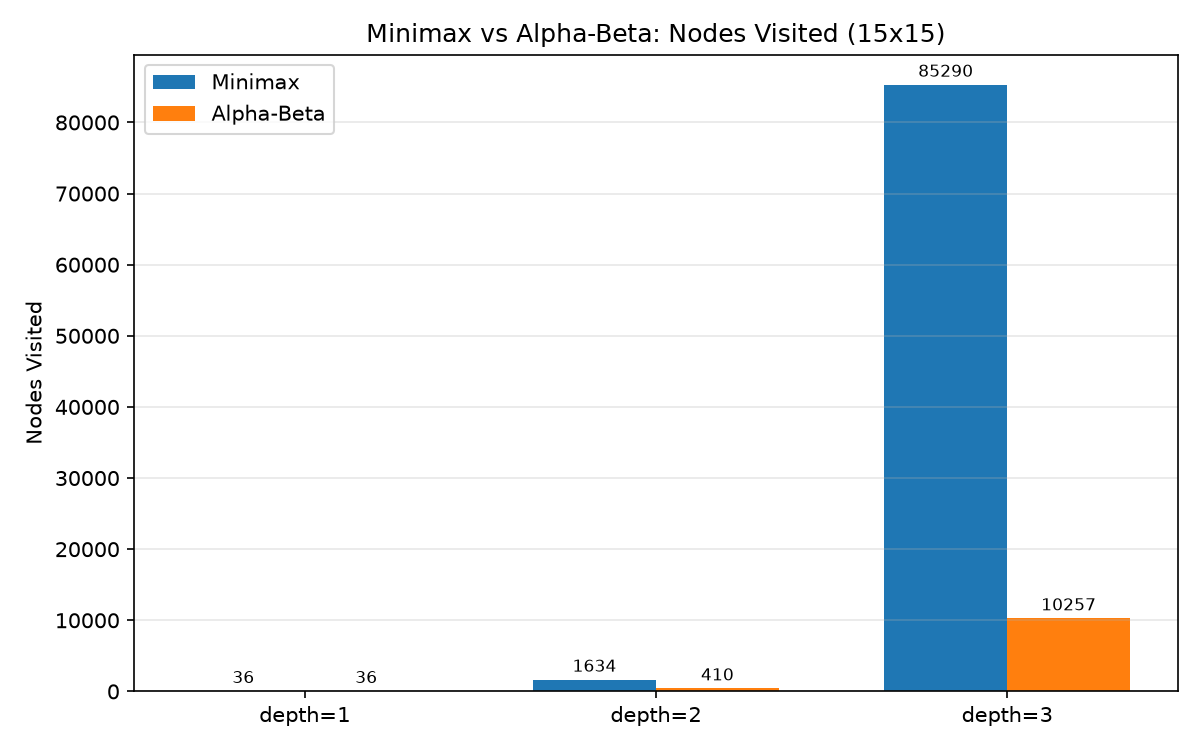
\includegraphics[width=0.95\linewidth]{../assets/figures/nodes_minimax_vs_ab_15x15.png}
\caption{So sánh số nút duyệt trên thế cờ khai cuộc $15\times 15$.}
\label{fig:nodes_15x15}
\end{figure}

\subsection{Kiểm chứng MCTS không bao giờ thua trên $3\times 3$}
Bảng~\ref{tab:never_lose} trình bày kết quả của MCTS-UCT khi đấu với đối thủ Alpha-Beta tối ưu ở độ sâu $9$ (duyệt hết toàn bộ cây trò chơi $3\times 3$) và đối thủ ngẫu nhiên qua $50$ ván đổi lượt mỗi cấu hình. Ở $100$ và $500$ vòng lặp, MCTS vẫn thua một số ván trước đối thủ tối ưu ($11/50$ và $2/50$ với $c=1{,}0$). Từ $1000$ vòng lặp trở lên, MCTS đạt \textbf{0 ván thua} ($50$ ván hòa) trước Alpha-Beta tối ưu, và đạt \textbf{0 ván thua} trước đối thủ ngẫu nhiên từ $500$ vòng lặp trở lên.

\begin{table}[t]
\centering
\caption{Kiểm chứng MCTS-UCT không thua trên $3\times 3$ (50 ván/cấu hình)}
\label{tab:never_lose}
\begin{tabular}{@{}lcrrrr@{}}
\toprule
Đối thủ & $c$ & Vòng lặp & Thắng & Hòa & Thua \\
\midrule
Alpha-Beta (d=9) & 1,0 & 100 & 0 & 39 & 11 \\
Alpha-Beta (d=9) & 1,0 & 500 & 0 & 48 & 2 \\
Alpha-Beta (d=9) & 1,0 & 1000 & 0 & 50 & \textbf{0} \\
Alpha-Beta (d=9) & 1,0 & 2000 & 0 & 50 & \textbf{0} \\
Alpha-Beta (d=9) & 1,414 & 100 & 0 & 41 & 9 \\
Alpha-Beta (d=9) & 1,414 & 500 & 0 & 48 & 2 \\
Alpha-Beta (d=9) & 1,414 & 1000 & 0 & 50 & \textbf{0} \\
Alpha-Beta (d=9) & 1,414 & 2000 & 0 & 50 & \textbf{0} \\
\midrule
Random & 1,0 & 100 & 46 & 2 & 2 \\
Random & 1,0 & 500 & 41 & 9 & \textbf{0} \\
Random & 1,0 & 1000 & 40 & 10 & \textbf{0} \\
Random & 1,0 & 2000 & 44 & 6 & \textbf{0} \\
Random & 1,414 & 100 & 44 & 2 & 4 \\
Random & 1,414 & 500 & 41 & 9 & \textbf{0} \\
Random & 1,414 & 1000 & 41 & 9 & \textbf{0} \\
Random & 1,414 & 2000 & 44 & 6 & \textbf{0} \\
\bottomrule
\end{tabular}
\end{table}

\subsection{Tỷ lệ thắng theo số vòng lặp ($3\times 3$ và $15\times 15$)}
Bảng~\ref{tab:mcts_3x3}--\ref{tab:mcts_15x15} và Hình~\ref{fig:winrate_3x3}--\ref{fig:winrate_15x15} thể hiện tỷ lệ thắng của MCTS trước tác tử ngẫu nhiên với $c \in \{0{,}5;\ 1{,}0;\ 1{,}4;\ 2{,}0\}$. Trên bàn $3\times 3$, cả bốn giá trị $c$ đều đạt $0$ ván thua khi $\text{iterations} \ge 500$, bão hòa quanh mức $84$--$90\%$ (các ván còn lại là hòa khi đi sau). Trên bàn $15\times 15$, $c = 0{,}5$ hội tụ nhanh nhất ở ngân sách thấp ($64{,}0\%$ ở $100$ vòng lặp, $100{,}0\%$ ở $200$ vòng lặp), trong khi ở $500$ vòng lặp cả $c = 1{,}0$ và $c = 1{,}4$ đều đạt $100{,}0\%$ ($50/50$).

\begin{table}[t]
\centering
\caption{Tỷ lệ thắng MCTS (\%) trên $3\times 3$ (100 ván/cấu hình)}
\label{tab:mcts_3x3}
\setlength{\tabcolsep}{3.5pt}
\begin{tabular}{@{}rcccccc@{}}
\toprule
$c$ & 50 & 100 & 200 & 500 & 1000 & 2000 \\
\midrule
0,5 & 82,0 & 81,0 & 91,0 & 89,0 & 87,0 & 87,0 \\
1,0 & 81,0 & 81,0 & 88,0 & 87,0 & 88,0 & 88,0 \\
1,4 & 87,0 & 90,0 & 84,0 & 86,0 & 84,0 & 90,0 \\
2,0 & 87,0 & 83,0 & 86,0 & 90,0 & 85,0 & 82,0 \\
\bottomrule
\end{tabular}
\end{table}

\begin{table}[t]
\centering
\caption{Tỷ lệ thắng MCTS (\%) trên $15\times 15$ (50 ván/cấu hình, T/H/B)}
\label{tab:mcts_15x15}
\begin{tabular}{@{}rcccc@{}}
\toprule
$c$ & 100 iters & 200 iters & 500 iters & ms/nước (500) \\
\midrule
0,5 & \textbf{64,0} (32/0/18) & \textbf{100,0} (50/0/0) & 98,0 (49/0/1) & 5.229 \\
1,0 & 54,0 (27/0/23) & 56,0 (28/0/22) & \textbf{100,0} (50/0/0) & 5.159 \\
1,4 & 52,0 (26/0/24) & 58,0 (29/0/21) & \textbf{100,0} (50/0/0) & 5.118 \\
2,0 & 46,0 (23/0/27) & 58,0 (29/0/21) & 96,0 (48/0/2) & 5.674 \\
\bottomrule
\end{tabular}
\end{table}

\begin{figure}[t]
\centering
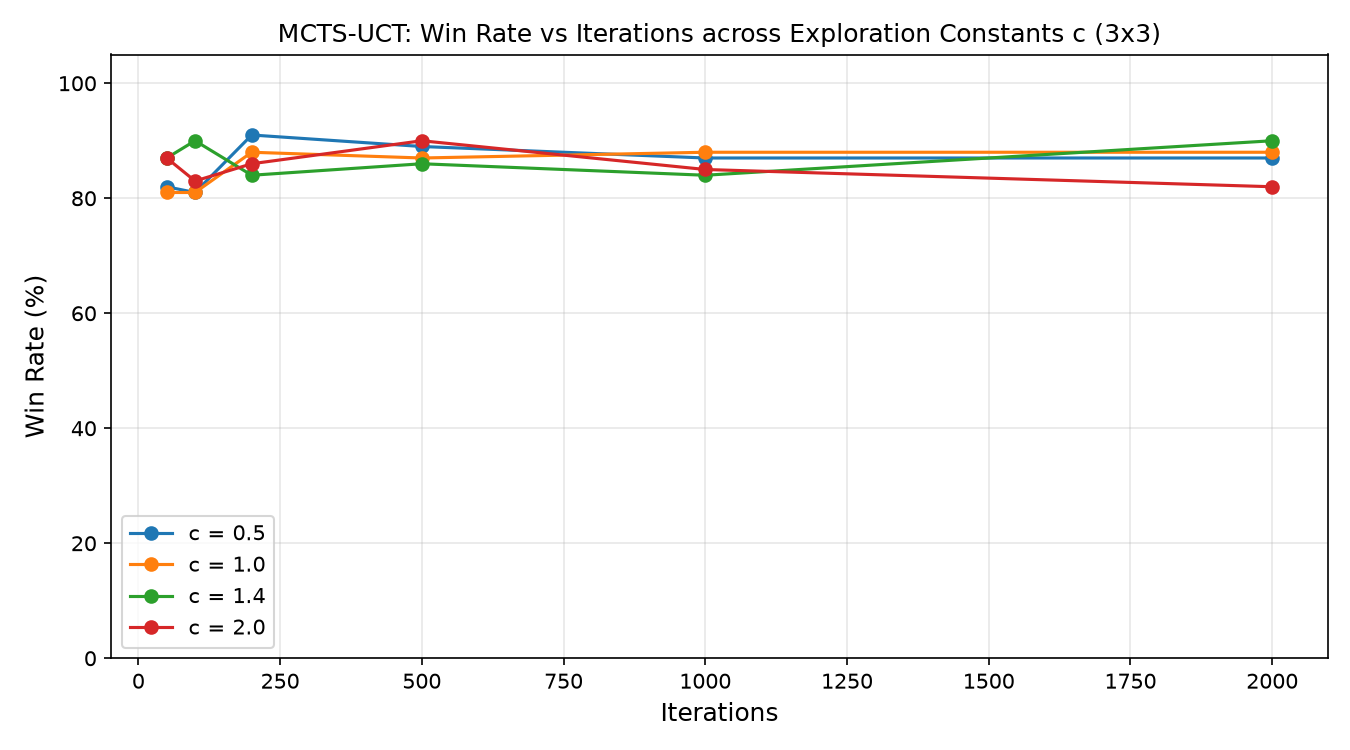
\includegraphics[width=0.95\linewidth]{../assets/figures/winrate_vs_iterations_3x3.png}
\caption{Tỷ lệ thắng MCTS-UCT theo số vòng lặp trên bàn $3\times 3$ (100 ván/cấu hình).}
\label{fig:winrate_3x3}
\end{figure}

\begin{figure}[t]
\centering
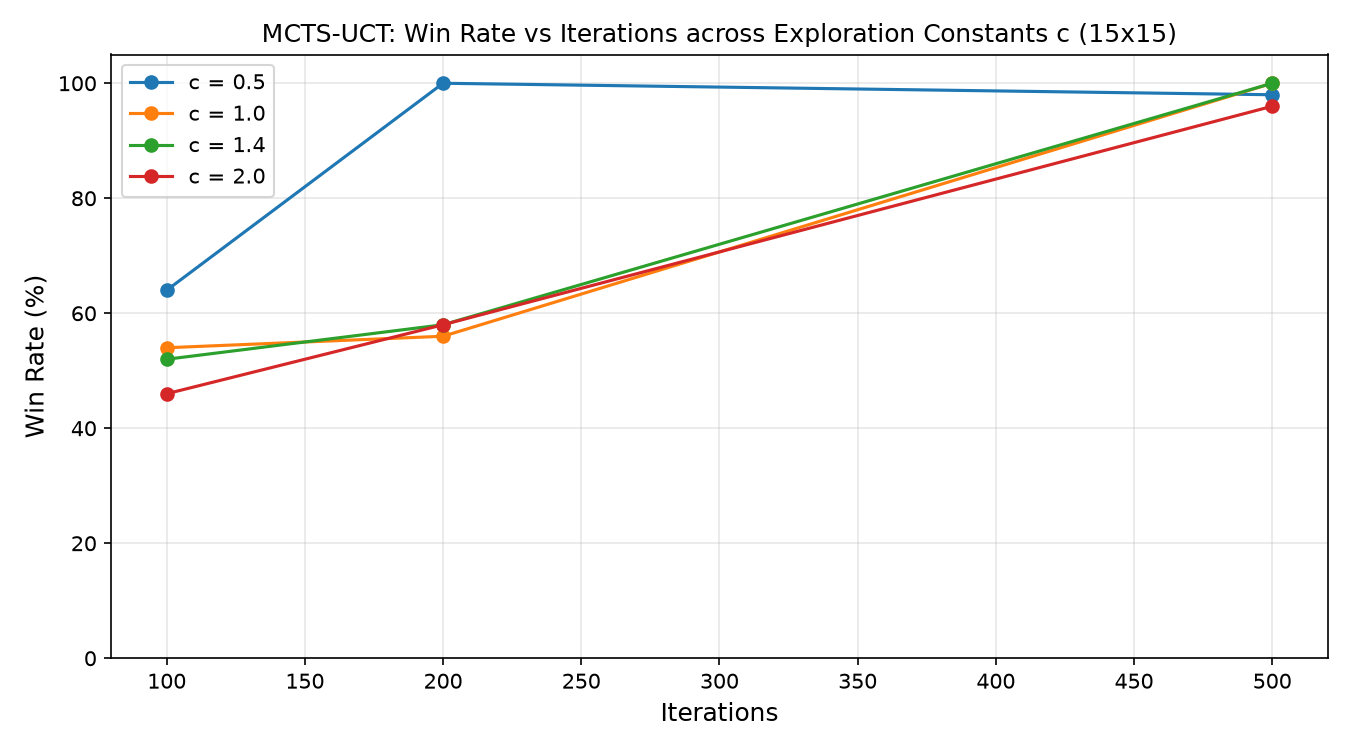
\includegraphics[width=0.95\linewidth]{../assets/figures/winrate_vs_iterations_15x15.png}
\caption{Tỷ lệ thắng MCTS-UCT theo số vòng lặp trên bàn $15\times 15$ (50 ván/cấu hình).}
\label{fig:winrate_15x15}
\end{figure}

\subsection{Thống kê tại nút gốc ($W$, $N$, $W/N$)}
Bảng~\ref{tab:root_stats} ghi lại thống kê các nút con gốc sau $1000$ vòng lặp ($c = 1{,}0$) trên thế cờ $3\times 3$ ($X$ tại $(1,1)$, $O$ tại $(0,0)$) và thế cờ khai cuộc $15\times 15$. Trên bàn $3\times 3$, UCT tập trung $545/1000$ lượt thăm vào hai nước mạnh nhất $(0,1)$ và $(1,0)$. Trên bàn $15\times 15$, do rollout ngẫu nhiên giới hạn $30$ bước hiếm khi kết thúc ở giai đoạn khai cuộc, các giá trị $W/N$ tập trung sát quanh $0{,}50$--$0{,}53$.

\begin{table}[t]
\centering
\caption{Thống kê tại nút gốc ($1000$ vòng lặp, $c = 1{,}0$)}
\label{tab:root_stats}
\begin{tabular}{@{}crrr|crrr@{}}
\toprule
\multicolumn{4}{c|}{Thế cờ $3\times 3$} & \multicolumn{4}{c}{Khai cuộc $15\times 15$ (Top 7)} \\
Nước & $W$ & $N$ & $W/N$ & Nước & $W$ & $N$ & $W/N$ \\
\midrule
(0, 1) & 242,5 & 299 & 0,811 & (5, 9) & 16,5 & 31 & 0,532 \\
(1, 0) & 195,0 & 246 & 0,793 & (10, 7) & 15,5 & 30 & 0,517 \\
(2, 0) & 87,0 & 121 & 0,719 & (5, 8) & 15,5 & 30 & 0,517 \\
(0, 2) & 80,0 & 112 & 0,714 & (10, 5) & 15,5 & 30 & 0,517 \\
(2, 1) & 56,0 & 83 & 0,675 & (4, 8) & 15,0 & 29 & 0,517 \\
(1, 2) & 50,5 & 77 & 0,656 & (5, 6) & 15,0 & 29 & 0,517 \\
(2, 2) & 39,0 & 62 & 0,629 & (8, 6) & 15,0 & 29 & 0,517 \\
\bottomrule
\end{tabular}
\end{table}

\subsection{Rollout ngẫu nhiên vs Rollout heuristic}
Bảng~\ref{tab:rollout} so sánh hai chiến lược rollout tại $c = \sqrt{2}$. Rollout heuristic cải thiện tỷ lệ thắng thêm $+6{,}0\%$ trên bàn $3\times 3$ và $+16{,}0\%$ trên bàn $15\times 15$, trong khi thời gian mỗi nước trên bàn $15\times 15$ chỉ tăng $1{,}52\times$ ($3.647 \rightarrow 5.553$~ms).

\begin{table}[t]
\centering
\caption{So sánh Rollout ngẫu nhiên và Rollout heuristic ($c = \sqrt{2}$)}
\label{tab:rollout}
\setlength{\tabcolsep}{4pt}
\begin{tabular}{@{}ccclrrr@{}}
\toprule
Bàn & Iters & Ván & Rollout & T/H/B & Thắng & ms/nước \\
\midrule
$3\times 3$ & 500 & 100 & Ngẫu nhiên & 84/16/0 & 84,0\% & 52,2 \\
$3\times 3$ & 500 & 100 & Heuristic & 90/10/0 & \textbf{90,0\%} & 51,2 \\
\midrule
$15\times 15$ & 200 & 50 & Ngẫu nhiên & 38/0/12 & 76,0\% & 3.647 \\
$15\times 15$ & 200 & 50 & Heuristic & 46/0/4 & \textbf{92,0\%} & 5.553 \\
\bottomrule
\end{tabular}
\end{table}

\subsection{Các biến thể công thức UCT và Progressive Bias}
Bảng~\ref{tab:uct_variants} và Hình~\ref{fig:uct_variants} so sánh bốn biến thể UCT cùng Progressive Bias tại $c = 1{,}0$. Việc bỏ $\ln$ (\texttt{no\_ln}) hoặc bỏ cả $\sqrt{\cdot}$ và $\ln$ (\texttt{linear}) làm tỷ lệ không thua trước Alpha-Beta tối ưu trên $3\times 3$ giảm từ $96{,}0\%$ xuống $76{,}0\%$ và $65{,}0\%$, đồng thời tỷ lệ thắng trên $15\times 15$ giảm từ $52{,}0\%$ xuống $34{,}0\%$. Ngược lại, Progressive Bias nâng tỷ lệ thắng trên $15\times 15$ ở $150$ vòng lặp từ $52{,}0\%$ lên \textbf{98,0\%} ($49/50$) và giảm thời gian trung bình mỗi nước ($2.709 \rightarrow 2.390$~ms).

\begin{table}[t]
\centering
\caption{So sánh các biến thể UCT và Progressive Bias ($c = 1{,}0$)}
\label{tab:uct_variants}
\scriptsize
\setlength{\tabcolsep}{2.5pt}
\begin{tabular}{@{}lccc@{}}
\toprule
Biến thể & $3\times 3$ vs AB (300) & $3\times 3$ vs Rand (200) & $15\times 15$ vs Rand (150) \\
 & Không thua (T/H/B) & Thắng / Không thua & Thắng (T/H/B) / ms \\
\midrule
UCT chuẩn & \textbf{96,0\%} (0/96/4) & 88,0\% / 98,0\% & 52,0\% (26/0/24) / 2.709 \\
Bỏ căn & 95,0\% (0/95/5) & 84,0\% / 99,0\% & 44,0\% (22/0/28) / 2.629 \\
Bỏ $\ln$ & 76,0\% (0/76/24) & 88,0\% / 97,0\% & 34,0\% (17/0/33) / 3.037 \\
Tuyến tính & 65,0\% (0/65/35) & 83,0\% / 93,0\% & 34,0\% (17/0/33) / 3.066 \\
\textbf{Prog.\ Bias} & 95,0\% (0/95/5) & \textbf{88,0\% / 100,0\%} & \textbf{98,0\%} (49/0/1) / \textbf{2.390} \\
\bottomrule
\end{tabular}
\end{table}

\begin{figure}[t]
\centering
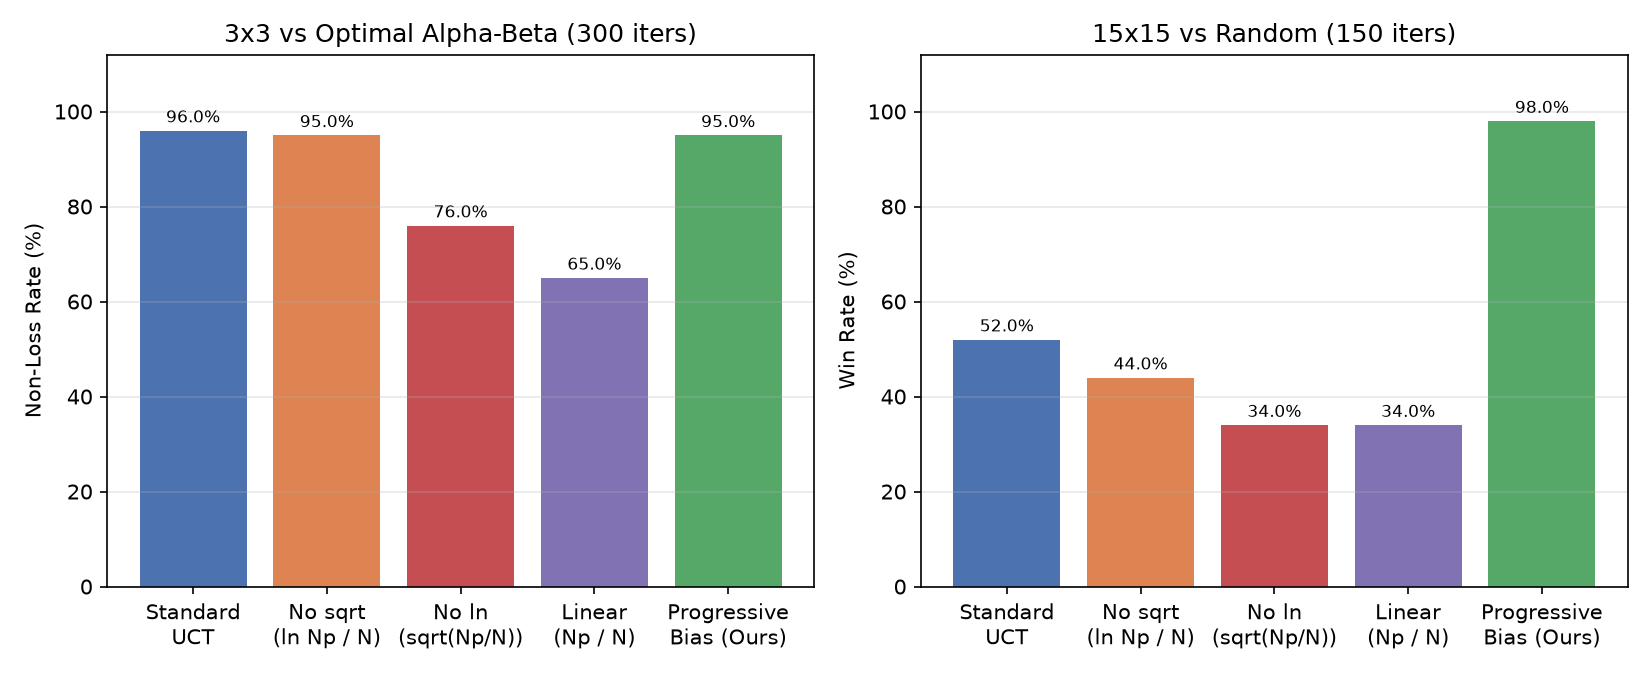
\includegraphics[width=0.98\linewidth]{../assets/figures/uct_variants_comparison.png}
\caption{So sánh các biến thể UCT và Progressive Bias trên $3\times 3$ (vs Alpha-Beta tối ưu) và $15\times 15$ (vs Random).}
\label{fig:uct_variants}
\end{figure}

\section{Thảo luận}

\textbf{RQ1 (Hiệu quả cắt tỉa Alpha-Beta):} Alpha-Beta cắt giảm $71{,}8\%$ số nút ở độ sâu $4$ trên bàn $3\times 3$ và $88{,}0\%$ ở độ sâu $3$ trên bàn $15\times 15$. Mức tiết kiệm tăng mạnh theo hệ số phân nhánh và độ sâu, lý giải vì sao Minimax thuần không thể dùng quá độ sâu $2$ trên bàn cờ caro $15\times 15$.

\textbf{RQ2 (Ảnh hưởng của hằng số khám phá $c$):} Trên bàn $3\times 3$, cả bốn giá trị $c$ đều đạt $0$ ván thua trước đối thủ ngẫu nhiên khi $\text{iterations} \ge 500$. Trên bàn $15\times 15$, sự đánh đổi giữa khám phá và khai thác thể hiện rõ ở ngân sách thấp: $c = 0{,}5$ hội tụ nhanh nhất ($64\%$ ở $100$ vòng lặp, $100\%$ ở $200$ vòng lặp), trong khi các giá trị $c$ lớn hơn dành nhiều vòng lặp đầu để thăm dò vùng lân cận rộng ($46$--$54\%$ ở $100$ vòng lặp). Khi đạt $500$ vòng lặp, cả bốn hằng số đều hội tụ lên $96$--$100\%$, với $c = 1{,}0$ và $c = 1{,}4$ đạt $100\%$ ($50/50$). Như vậy, $c$ nhỏ ($0{,}5$) phù hợp khi ngân sách vòng lặp hạn chế trên bàn lớn, còn $c \in [1{,}0;\ 1{,}4]$ tối ưu khi có đủ ngân sách.

\textbf{RQ3 (Tính chất không thua trên $3\times 3$):} Khi đấu với Alpha-Beta tối ưu ở độ sâu $9$, MCTS vẫn thua một số ván ở ngân sách thấp ($11/50$ ván thua ở $100$ vòng lặp, $2/50$ ở $500$ vòng lặp với $c = 1{,}0$) do cây nông bỏ sót các thế cờ đôi bắt buộc. Từ $\text{iterations} \ge 1000$ trở đi, MCTS đạt $0$ ván thua trên $50$ ván ($50$ ván hòa) cho cả $c = 1{,}0$ và $c = 1{,}414$, kiểm chứng thực nghiệm sự hội tụ lý thuyết của UCT trên Tic-Tac-Toe $3\times 3$.

\textbf{RQ4 (Rollout heuristic và liên hệ với Value Network):} Thay thế rollout ngẫu nhiên bằng heuristic thắng/chặn một bước giúp tăng tỷ lệ thắng $+6{,}0\%$ trên $3\times 3$ và $+16{,}0\%$ trên $15\times 15$ với chi phí thời gian chỉ tăng $1{,}52\times$ nhờ kiểm tra trực tiếp trên bàn cờ mà không sao chép đối tượng. Ngay cả một bộ lọc chiến thuật nông cũng giảm đáng kể nhiễu mô phỏng trên bàn lớn. Điều này phản ánh bước tiến từ MCTS cổ điển sang AlphaGo/AlphaZero~\cite{silver2016}, nơi mạng chính sách và mạng giá trị học sâu thay thế các lượt rollout nhiễu bằng đánh giá trực tiếp trạng thái và phân phối xác suất nước đi.

\textbf{RQ5 (Chọn nước theo $N$ thay vì $W/N$):} Khi kết thúc tìm kiếm, \texttt{get\_move()} chọn \texttt{most\_visited\_child()} ($N$ lớn nhất) thay vì $W/N$ lớn nhất. Một nút con ít được thăm có thể có $W/N$ cao giả tạo (ví dụ $1{,}0$ sau $1$--$2$ lần mô phỏng may mắn) do phương sai lấy mẫu lớn. Vì UCT phân bổ lượt thăm tiệm cận theo chất lượng thực của nhánh, nút được thăm nhiều nhất vừa có khoảng tin cậy hẹp nhất vừa là ước lượng ổn định nhất.

\textbf{RQ6 (Biến thể UCT \& Progressive Bias):} Việc bỏ $\ln$ (\texttt{no\_ln}) hoặc bỏ cả $\sqrt{\cdot}$ và $\ln$ (\texttt{linear}) khiến số hạng khám phá tăng theo đa thức của $N_{\mathrm{parent}}$, làm UCT không tập trung được vào các nhánh mạnh ($96{,}0\% \rightarrow 76{,}0\% / 65{,}0\%$ không thua trên $3\times 3$; $52{,}0\% \rightarrow 34{,}0\%$ thắng trên $15\times 15$). Chỉ bỏ $\sqrt{\cdot}$ (\texttt{no\_sqrt}) phạt quá nặng các nút ít thăm và làm tỷ lệ thắng trên $15\times 15$ giảm còn $44{,}0\%$. Ngược lại, bổ sung Progressive Bias ($H_i/(N_i+1)$) nâng tỷ lệ thắng trên $15\times 15$ ở $150$ vòng lặp từ $52{,}0\%$ lên $98{,}0\%$ ($+46{,}0\%$) đồng thời giảm thời gian mỗi nước ($2.709 \rightarrow 2.390$~ms) do ván đấu kết thúc sớm hơn.

\textbf{Hạn chế:} (1) Trên bàn $15\times 15$, giới hạn rollout ở $30$ bước giúp thời gian chạy khả thi nhưng khiến phần lớn mô phỏng ở khai cuộc dừng ở trạng thái chưa phân thắng bại ($0{,}5$), làm giá trị $W/N$ tại gốc dồn quanh $0{,}50$--$0{,}53$ (Bảng~\ref{tab:root_stats}); dùng \texttt{evaluate()} chấm điểm khi cắt rollout sẽ cho tín hiệu mạnh hơn. (2) \texttt{MCTSAgent} dựng lại cây từ đầu ở mỗi nước đi (chưa tái sử dụng cây), và \texttt{Board.get\_legal\_moves()} tính lại vùng lân cận bán kính $2$ từ \texttt{move\_history} ở mỗi lần gọi. (3) Alpha-Beta độ sâu $3$ trên $15\times 15$ chưa có sắp xếp nước đi (move ordering) và chưa nhận diện đòn đôi trong \texttt{evaluate()}, nên vẫn dễ bị bẫy nhiều nước.

\section{Kết luận}
Chúng tôi đã cài đặt và đánh giá Minimax cắt tỉa Alpha-Beta cùng MCTS-UCT trên Tic-Tac-Toe $3\times 3$ và $15\times 15$. Alpha-Beta cắt giảm $71{,}8\%$ số nút trên $3\times 3$ (độ sâu $4$) và $88{,}0\%$ trên $15\times 15$ (độ sâu $3$). Trên bàn $3\times 3$, MCTS-UCT đạt $0$ ván thua trước cả đối thủ ngẫu nhiên ($\ge 500$ vòng lặp) lẫn Alpha-Beta tối ưu độ sâu $9$ ($\ge 1000$ vòng lặp). Trên bàn $15\times 15$, $c = 0{,}5$ hội tụ nhanh nhất ở ngân sách thấp ($100\%$ ở $200$ vòng lặp), trong khi $c \in \{1{,}0;\ 1{,}4\}$ đạt $100\%$ ($50/50$) ở $500$ vòng lặp. Cuối cùng, rollout heuristic một bước giúp tăng tỷ lệ thắng $+6{,}0\%$ trên $3\times 3$ và $+16{,}0\%$ trên $15\times 15$, minh họa trực giác cốt lõi đằng sau mạng giá trị và mạng chính sách trong AI trò chơi hiện đại.

\begin{thebibliography}{00}
\bibitem{auer2002} P. Auer, N. Cesa-Bianchi, and P. Fischer, ``Finite-time analysis of the multiarmed bandit problem,'' \emph{Machine Learning}, vol. 47, no. 2--3, pp. 235--256, 2002.
\bibitem{kocsis2006} L. Kocsis and C. Szepesv\'ari, ``Bandit based Monte-Carlo planning,'' in \emph{Proc. ECML}, 2006, pp. 282--293.
\bibitem{coulom2006} R. Coulom, ``Efficient selectivity and backup operators in Monte-Carlo tree search,'' in \emph{Proc. ICCG}, 2006, pp. 72--83.
\bibitem{silver2016} D. Silver et al., ``Mastering the game of Go with deep neural networks and tree search,'' \emph{Nature}, vol. 529, pp. 484--489, 2016.
\bibitem{chaslot2008} G. M. J.-B. Chaslot, M. H. M. Winands, H. J. van den Herik, J. W. H. M. Uiterwijk, and B. Bouzy, ``Progressive strategies for Monte-Carlo tree search,'' \emph{New Mathematics and Natural Computation}, vol. 4, no. 3, pp. 343--357, 2008.
\bibitem{russell2020} S. Russell and P. Norvig, \emph{Artificial Intelligence: A Modern Approach}, 4th ed. Pearson, 2020.
\end{thebibliography}

\end{document}
